\chapter{Lahir, Tumbuh, Mati}\label{ch:g2:born-grow-die}

Pada musim semi, pohon ceri di dekat gerbang tertutup \omterm{def:g1:plants-around-us:parts}{bunga}; di
bawahnya, seekor kucing menyusui anak-anaknya yang baru lahir; dan
Kakek memperlihatkan foto dirinya ketika seusia kamu --- kecil, ompong,
dan sudah gemar buah ceri. Setiap \omterm{def:g1:living-or-not:living}{makhluk hidup} menempuh jalan yang
sama: ia bermula, ia tumbuh, dan pada suatu hari ia berakhir. Jalan
itu disebut \omterm{def:g2:born-grow-die:cycle}{daur hidup}.

\section{Tahap-tahap sebuah kehidupan}

\begin{definition}[Daur hidup]\label{def:g2:born-grow-die:cycle}
Yang disebut \emph{daur hidup}\index{daur hidup} sebuah \omterm{def:g1:living-or-not:living}{makhluk hidup}
adalah deretan \emph{tahap}\index{tahap} yang dilalui hidupnya:
\begin{enumerate}
  \item ia \emph{lahir}\index{kelahiran} --- permulaannya;
  \item ia masih \emph{muda}\index{muda} --- ia tumbuh dan berubah
        dengan cepat;
  \item ia \emph{dewasa}\index{dewasa} --- tumbuh penuh; yang dewasa
        dapat mempunyai anak sendiri;
  \item ia menjadi \emph{tua}\index{usia tua}, dan pada akhirnya ia
        \emph{mati}\index{kematian}.
\end{enumerate}
\end{definition}

\begin{example}[Tiga kehidupan, satu jalan]\label{ex:g2:born-grow-die:three}
Seekor anak kucing lahir, bermain lalu tumbuh menjadi kucing, yang
kelak dapat punya anak sendiri, lalu menjadi tua. Sebutir biji ceri
berkecambah, pohon mudanya bertambah tinggi bertahun-tahun, pohon
\omterm{def:g2:born-grow-die:cycle}{dewasanya} membuat \omterm{def:g1:plants-around-us:parts}{bunga} dan buah ceri, dan sesudah berpuluh-puluh
tahun ia mati. Dan kamu: bayi, anak, lalu pada suatu hari orang
\omterm{def:g2:born-grow-die:cycle}{dewasa}. Anak kucing, pohon ceri, anak manusia --- empat \omterm{def:g2:born-grow-die:cycle}{tahap} yang
sama.
\end{example}

\begin{omfigure}
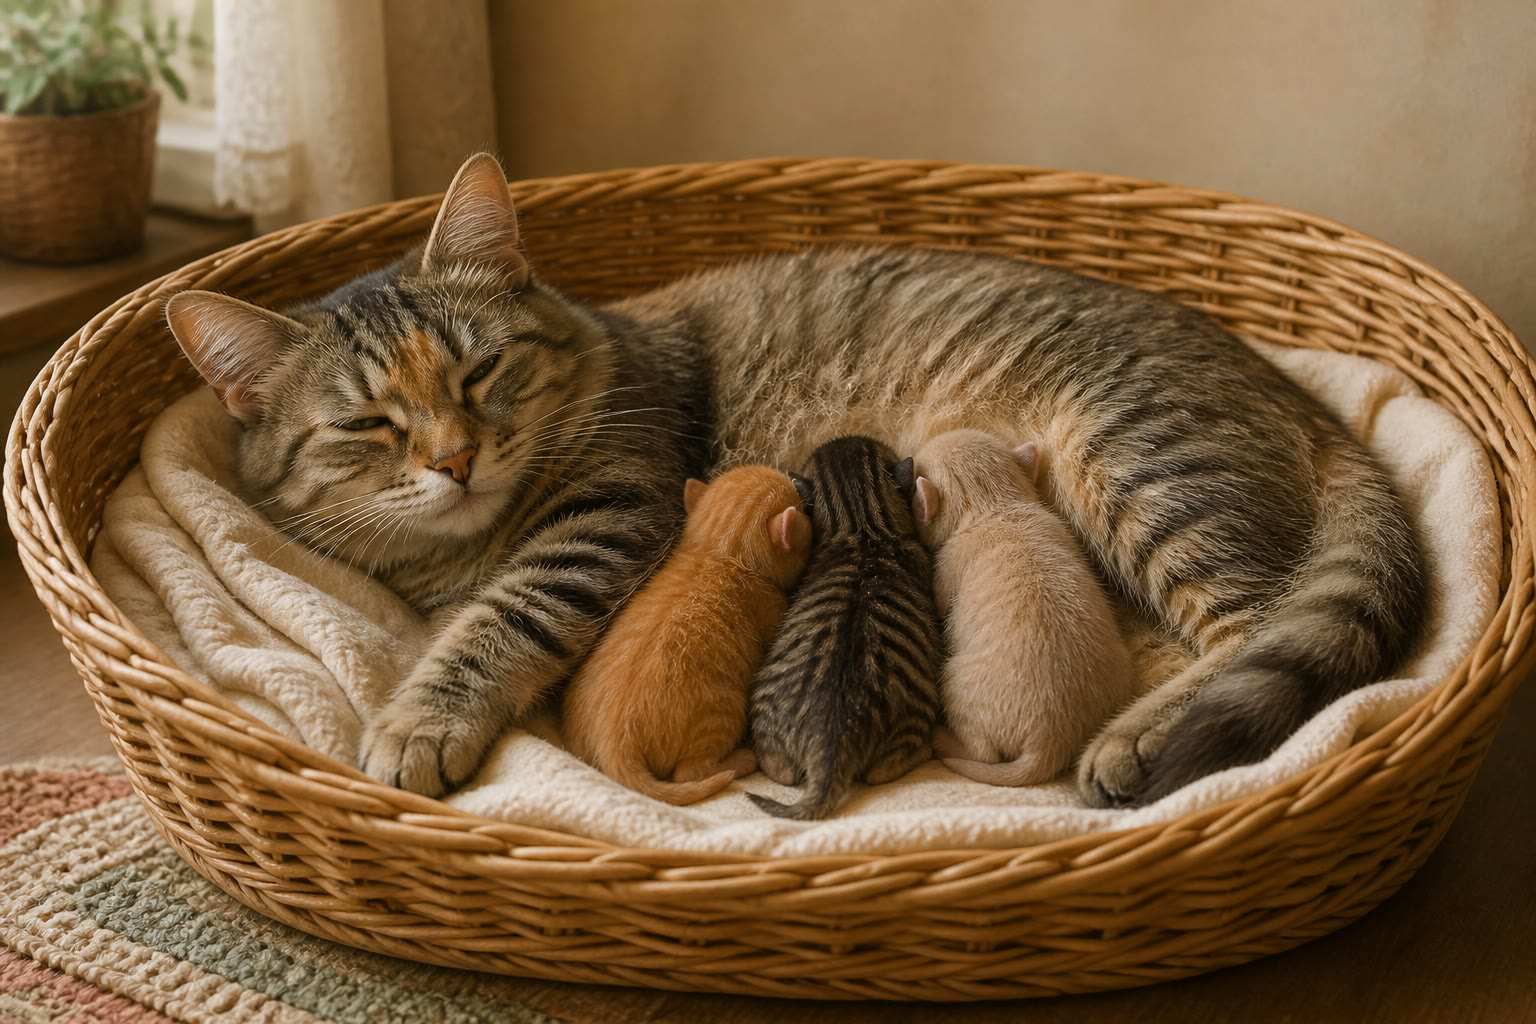
\includegraphics[width=0.62\linewidth]{images/book1/ai/g2-cycle-kittens.jpg}

{\small Permulaan tiga \omterm{def:g2:born-grow-die:cycle}{daur hidup} sekaligus: anak-anak kucing yang
baru lahir pada susu induknya.}
\end{omfigure}

\begin{omfigure}
\begin{tikzpicture}[scale=0.92]
  \foreach \x/\txt in {0/{lahir},3.1/{muda},6.2/{dewasa},9.3/{usia tua}} {
    \draw[thick, omDef, fill=omDef!7, rounded corners=5pt]
      (\x,0) rectangle ({\x+2.4},1.2);
    \node[font=\small\bfseries, text height=1.6ex, text depth=0.4ex]
      at ({\x+1.2},0.6) {\txt};
  }
  \draw[->, thick, omMeth] (2.4,0.6) -- (3.1,0.6);
  \draw[->, thick, omMeth] (5.5,0.6) -- (6.2,0.6);
  \draw[->, thick, omMeth] (8.6,0.6) -- (9.3,0.6);
  % new generation arrow
  \draw[->, thick, omProp] (7.4,1.2) .. controls (7.4,2.3) and (1.2,2.3)
    .. (1.2,1.25);
  \node[font=\small, omProp] at (4.3,2.35) {yang dewasa punya anak: daur baru bermula};
\end{tikzpicture}

{\small \omterm{def:g2:born-grow-die:cycle}{Tahap-tahap} sebuah kehidupan --- dan anak panah yang memulai
jalan itu lagi bersama generasi berikutnya.}
\end{omfigure}

\begin{remark}[Mengapa disebut daur]\label{rem:g2:born-grow-die:wheel}
Tiap kehidupan tunggal berjalan dari \omterm{def:g2:born-grow-die:cycle}{kelahiran} sampai kematian,
seperti jalan dengan dua ujung. Tetapi sebelum ujungnya, yang \omterm{def:g2:born-grow-die:cycle}{dewasa}
punya anak, dan anak-anak itu memulai jalannya lagi. Dilihat sepanjang
banyak generasi, kehidupan berputar seperti roda --- itulah sebabnya
kita menyebutnya \emph{daur} hidup.
\end{remark}

\section{Tumbuh dan berubah}

\begin{proposition}[Bertambah besar bukan satu-satunya]\label{prop:g2:born-grow-die:change}
Sambil tumbuh, \omterm{def:g1:living-or-not:living}{makhluk hidup} yang muda juga \emph{berubah}: seorang
bayi tumbuh gigi, menanggalkannya, lalu mendapat gigi yang lebih kuat;
\omterm{def:g1:animals-around-us:covering}{bulu} kuning seekor anak ayam menjadi \omterm{def:g1:animals-around-us:covering}{bulu burung} yang sesungguhnya;
\omterm{def:g1:plants-around-us:parts}{batang} hijau yang lunak pada pohon muda berubah menjadi kayu yang
keras. Tumbuh berarti bertambah besar \emph{dan} menjadi berbeda.
\end{proposition}
\admitted

\begin{example}[Ujian foto]\label{ex:g2:born-grow-die:photo}
Pada foto-foto lama Kakek kamu dapat mengikuti satu orang melewati
setiap \omterm{def:g2:born-grow-die:cycle}{tahap}: bayi, anak sekolah, pemuda, ayah, kakek. Orang yang
sama, tubuh yang berubah. Foto adalah mesin waktu kecil untuk
mengamati sebuah \omterm{def:g2:born-grow-die:cycle}{daur hidup}.
\end{example}

\begin{method}[Mengurutkan tahap kehidupan]\label{met:g2:born-grow-die:order}
Diberikan gambar-gambar kehidupan sebuah \omterm{def:g1:living-or-not:living}{makhluk hidup}, dalam keadaan
teracak:
\begin{enumerate}
  \item temukan gambar \omterm{def:g2:born-grow-die:cycle}{kelahirannya} --- telur, biji atau bayi yang
        baru lahir;
  \item temukan yang \omterm{def:g2:born-grow-die:cycle}{dewasa} --- tumbuh penuh, mampu punya anak;
  \item letakkan yang muda di antaranya, dari yang lebih kecil ke yang
        lebih besar;
  \item periksa deretanmu: apakah tiap gambar mengantar ke gambar
        berikutnya?
\end{enumerate}
\end{method}

\section{Setiap kehidupan berakhir --- dan kehidupan berlanjut}

\begin{proposition}[Rentang hidup]\label{prop:g2:born-grow-die:lifespan}
\omterm{def:g1:living-or-not:living}{Makhluk hidup} yang berbeda hidup dalam lama waktu yang berbeda ---
sebuah \emph{rentang hidup}\index{rentang hidup}. Seekor kupu-kupu
mungkin hidup beberapa minggu; seekor kucing, dan seekor anjing,
sepuluh sampai dua puluh tahun; seorang manusia sering lebih dari
delapan puluh tahun; sebagian pohon, ratusan tahun. Panjang atau
pendek, setiap kehidupan mempunyai akhir.
\end{proposition}
\admitted

\begin{example}[Pohon apel yang tua]\label{ex:g2:born-grow-die:oldtree}
Pohon apel tua yang bengkok di ujung kebun memberi buah makin sedikit
tiap tahun --- ia sedang berada di \omterm{def:g2:born-grow-die:cycle}{usia tuanya}. Tetapi apelnya
berbiji, dan satu biji, kalau ditanam, sudah merupakan pohon apel muda
yang memulai jalannya. Ketika pohon tuanya mati, pohon apel tidak akan
lenyap: anak-anaknya meneruskan.
\end{example}

\begin{remark}[Berbicara tentang kematian]\label{rem:g2:born-grow-die:death}
Mati adalah bagian dari setiap \omterm{def:g2:born-grow-die:cycle}{daur hidup}, dan wajar saja merasa sedih
karenanya --- orang memang begitu, terutama tentang \omterm{def:g1:animals-around-us:animal}{hewan} peliharaan
dan tentang orang yang kita sayangi. \omterm{def:g1:living-or-not:living}{Biologi} menambahkan satu
penghiburan: karena yang \omterm{def:g2:born-grow-die:cycle}{dewasa} punya anak sebelum mereka mati,
kehidupan itu sendiri berlanjut, daur demi daur.
\end{remark}

\section{Latihan}

\begin{exercise}[$\star$]\label{exo:g2:born-grow-die:1}
Sebutkan keempat \omterm{def:g2:born-grow-die:cycle}{tahap} sebuah \omterm{def:g2:born-grow-die:cycle}{daur hidup}, berurutan.
\end{exercise}

\begin{exercise}[$\star$]\label{exo:g2:born-grow-die:2}
Pada \omterm{def:g2:born-grow-die:cycle}{tahap} mana sebuah \omterm{def:g1:living-or-not:living}{makhluk hidup} dapat punya anak sendiri?
\end{exercise}

\begin{exercise}[$\star$]\label{exo:g2:born-grow-die:3}
Urutkan dari yang paling tua ke yang paling muda: seorang anak
sekolah, seorang bayi, seorang nenek, seorang ibu.
\end{exercise}

\begin{exercise}[$\star$]\label{exo:g2:born-grow-die:4}
Sebutkan \omterm{def:g2:born-grow-die:cycle}{daur hidup} pohon ceri pada
\cref{ex:g2:born-grow-die:three}, \omterm{def:g2:born-grow-die:cycle}{tahap} demi \omterm{def:g2:born-grow-die:cycle}{tahap}.
\end{exercise}

\begin{exercise}[$\star$]\label{exo:g2:born-grow-die:5}
Berikan dua contoh dari \cref{prop:g2:born-grow-die:change} tentang
\omterm{def:g1:living-or-not:living}{makhluk hidup} muda yang \emph{berubah} sambil tumbuh, bukan sekadar
bertambah besar.
\end{exercise}

\begin{exercise}[$\star$]\label{exo:g2:born-grow-die:6}
Siapa yang biasanya hidup lebih lama: kupu-kupu, kucing, atau pohon
ek? Urutkan ketiganya menurut \omterm{prop:g2:born-grow-die:lifespan}{rentang hidupnya}.
\end{exercise}

\begin{exercise}[$\star$]\label{exo:g2:born-grow-die:7}
Mengapa dipakai kata \emph{daur}, padahal tiap kehidupan tunggal
berjalan dari \omterm{def:g2:born-grow-die:cycle}{kelahiran} sampai kematian seperti sebuah jalan? Pakai
anak panah ungu pada gambarnya.
\end{exercise}

\begin{exercise}[$\star$]\label{exo:g2:born-grow-die:8}
Cobalah: mintalah kepada keluargamu foto-foto seorang \omterm{def:g2:born-grow-die:cycle}{dewasa} pada
berbagai usia, lalu urutkan menurut \omterm{def:g2:born-grow-die:cycle}{daur hidup} dengan
\cref{met:g2:born-grow-die:order}. \omterm{def:g2:born-grow-die:cycle}{Tahap} mana saja yang diperlihatkan
foto-foto itu? \omterm{def:g2:born-grow-die:cycle}{Tahap} mana yang masih akan datang?
\end{exercise}

\begin{exercise}[$\star\star$]\label{exo:g2:born-grow-die:9}
Pohon apel tua pada \cref{ex:g2:born-grow-die:oldtree} akan mati pada
suatu hari, namun kebunnya tidak harus kehilangan pohon apelnya.
Jelaskan mengapa, dengan kata \emph{generasi} atau dengan anak panah
ungu pada gambarnya.
\end{exercise}

\begin{exercise}[$\star\star$]\label{exo:g2:born-grow-die:10}
Sebutir kerikil tidak pernah mati. Apakah itu karena ia sangat kuat?
Pakai gagasan hidup dan tak hidup pada
\cref{ch:g1:living-or-not} untuk menjelaskannya.
\end{exercise}
